\documentclass[sigconf,nonacm]{acmart}

\settopmatter{printacmref=false}
\renewcommand\footnotetextcopyrightpermission[1]{}

\usepackage{booktabs}
\usepackage{tikz}
\usepackage{xspace}
\usetikzlibrary{arrows.meta,positioning,fit,shapes.geometric}

\newcommand{\briskstate}{BriskState\xspace}

\title{Demonstrating \briskstate: A Cache-Aware State Backend for Apache Flink}

\author{Anonymous Authors}
\affiliation{%
  \institution{Anonymous Submission}%
  \city{Anonymous}%
  \country{Anonymous}%
}

\begin{document}

\begin{abstract}
Stateful stream processing often becomes memory-bound before it becomes compute-bound. Frequent state lookups, window maintenance, and timer firing amplify cache misses, long object-indirection chains, and heap-management overhead, yet these effects are hard to observe in a live system. This paper presents a demonstration of \briskstate, an Apache Flink state backend together with its native execution engine and the existing WordCount and NexMark benchmark artifacts in the repository. The goal is to expose the backend design itself: compact state organization, locality-aware access paths, and their impact on throughput, latency, checkpoint behavior, and state-access hot spots during live runs and trace replay. A lightweight interface is used only to make these behaviors observable and to support side-by-side comparison against heap-based baselines. The paper focuses on how the \briskstate design appears in execution traces and how locality-aware storage changes runtime symptoms in state-intensive stream-processing workloads.
\end{abstract}

\keywords{stream processing, state backend, \briskstate, cache-aware data layout, Apache Flink}

\maketitle

\section{Introduction}
Large-state stream-processing pipelines rely on the state backend on nearly every record. In Apache Flink, this path is exercised by point updates, window aggregation, joins, and timer callbacks, so backend behavior can dominate end-to-end performance even when user logic is lightweight \cite{carbone2015flink}. In practice, the bottleneck is frequently the memory hierarchy rather than arithmetic throughput: state accesses trigger pointer chasing, touch multiple cache lines, and create runtime jitter through heap-management activity.

Conventional benchmark plots show final throughput or completion time, yet they do not show why one backend stalls, which namespaces become hot, or how checkpoint traffic and key-group locality change over time. The missing link is the execution evidence needed to connect backend structure with observed runtime behavior.

\briskstate addresses this gap with a cache-aware backend integrated with the delivered benchmark harness. The backend follows the implemented Java-control-layer, JNI-bridge, and native-engine split described in the project documentation, while a lightweight interface exposes the resulting behavior through a control panel, topology and state inspector, and time-series views for throughput, latency, and checkpoint activity. The workflow covers both pure state-stress workloads and realistic streaming jobs within a single experimental path.

\briskstate is positioned against three nearby lines of work. Stateful dataflow systems such as MillWheel, Flink, Naiad, Structured Streaming, and the Dataflow model define high-level execution semantics, but the physical organization of state remains largely hidden behind operator APIs and runtime services \cite{akidau2013millwheel,carbone2015flink,murray2013naiad,armbrust2018structured,akidau2015dataflow}. In Flink deployments, backend choices usually reduce to in-memory heap structures or embedded persistent stores such as RocksDB, while work on consistent state management and migration, including Flink state management and Megaphone, emphasizes correctness and continuity rather than layout-aware observability \cite{carbone2015flink,rocksdb,carbone2017statemanagement,hoffman2019megaphone}. High-performance key-value engines and compact hash-table designs, including FASTER and Swiss-table-style indexing, show that memory layout and probing discipline materially change access cost, and benchmark suites such as NexMark capture the resulting end-to-end outcomes without exposing the runtime state structure behind them \cite{chandramouli2018faster,abseil2018swisstable,tucker2008nexmark}. \briskstate targets that gap by making a Flink-compatible state backend observable as a running systems component rather than evaluating it only through final aggregate scores.

The paper makes three contributions:
\begin{itemize}
  \item It presents \briskstate together with a runnable workflow for comparing it against standard heap-based baselines under the same Flink workloads.
  \item It exposes otherwise hidden structures, including key-group routing, namespace occupancy, and checkpoint phases, so locality effects become understandable during execution.
  \item It packages the current \briskstate prototype, benchmark harness, and observation workflow into a reproducible demonstration based on standard Linux deployment.
\end{itemize}

\section{\briskstate}
\subsection{Overview}
Figure~\ref{fig:architecture} summarizes the demonstration architecture. The control plane accepts workload and backend selections from the web interface, launches the requested Flink job, and subscribes to runtime metrics emitted by the benchmark harness, Flink runtime, and lightweight collectors. The data plane runs the target job with either a heap-based baseline or \briskstate, then streams summarized metrics and structural summaries back to the interface.

\begin{figure}[t]
  \centering
  \resizebox{\columnwidth}{!}{%
  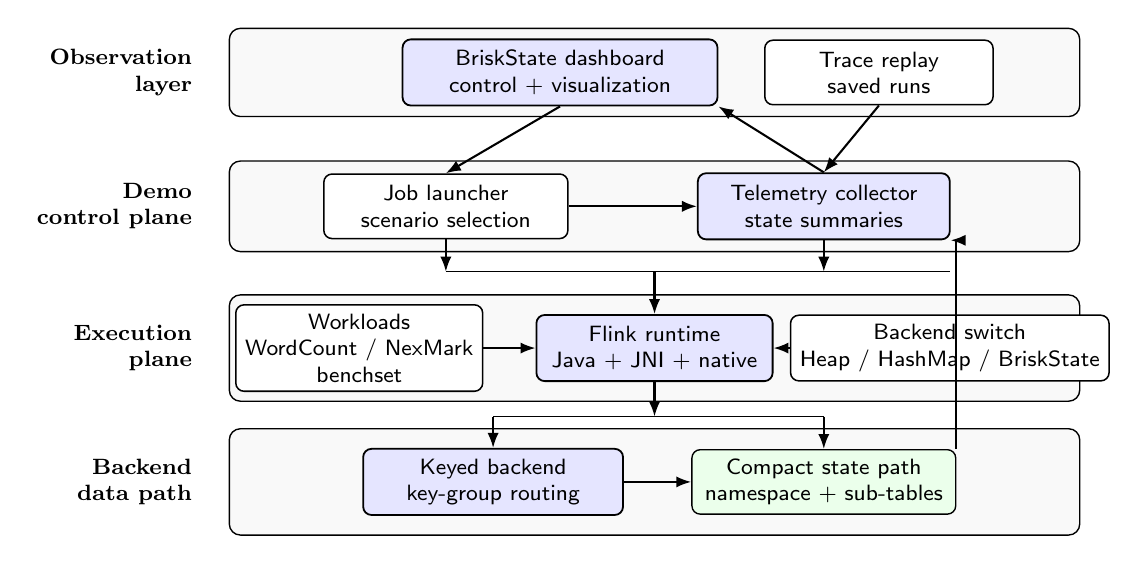
\begin{tikzpicture}[
      x=1cm,
      y=1cm,
      font=\footnotesize\sffamily,
      lane/.style={draw, rounded corners=4pt, line width=0.5pt, fill=gray!5},
      figtitle/.style={font=\footnotesize\bfseries, align=right},
      box/.style={draw, rounded corners=3pt, line width=0.55pt, align=center, fill=white, minimum height=0.82cm},
      accentbox/.style={draw, rounded corners=3pt, line width=0.65pt, align=center, fill=blue!10, minimum height=0.84cm},
      subtlebox/.style={draw, rounded corners=3pt, line width=0.5pt, align=center, fill=green!8, minimum height=0.8cm},
      line/.style={-{Latex[length=1.9mm]}, line width=0.75pt},
      thinline/.style={line width=0.45pt}
    ]
    \node[figtitle, anchor=east] at (1.45,5.95) {Observation\\layer};
    \node[figtitle, anchor=east] at (1.45,4.25) {Demo\\control plane};
    \node[figtitle, anchor=east] at (1.45,2.45) {Execution\\plane};
    \node[figtitle, anchor=east] at (1.45,0.75) {Backend\\data path};

    \node[lane, minimum width=10.8cm, minimum height=1.12cm] at (7.2,5.95) {};
    \node[lane, minimum width=10.8cm, minimum height=1.15cm] at (7.2,4.25) {};
    \node[lane, minimum width=10.8cm, minimum height=1.35cm] at (7.2,2.45) {};
    \node[lane, minimum width=10.8cm, minimum height=1.35cm] at (7.2,0.75) {};

    \node[accentbox, minimum width=4.0cm] (ui) at (6.0,5.95) {\briskstate dashboard\\control + visualization};
    \node[box, minimum width=2.9cm] (replay) at (10.05,5.95) {Trace replay\\saved runs};

    \node[box, minimum width=3.1cm] (launcher) at (4.55,4.25) {Job launcher\\scenario selection};
    \node[accentbox, minimum width=3.2cm] (controller) at (9.35,4.25) {Telemetry collector\\state summaries};

    \node[box, minimum width=2.55cm] (workload) at (3.45,2.45) {Workloads\\WordCount / NexMark\\benchset};
    \node[accentbox, minimum width=3.0cm] (runtime) at (7.2,2.45) {Flink runtime\\Java + JNI + native};
    \node[box, minimum width=2.85cm] (backend) at (10.95,2.45) {Backend switch\\Heap / HashMap / \briskstate};

    \node[accentbox, minimum width=3.3cm] (state) at (5.15,0.75) {Keyed backend\\key-group routing};
    \node[subtlebox, minimum width=3.35cm] (table) at (9.35,0.75) {Compact state path\\namespace + sub-tables};

    \draw[line] (ui.south) -- (launcher.north);
    \draw[line] (replay.south) -- (controller.north);
    \draw[line] (launcher.east) -- (controller.west);

    \coordinate (busA) at (7.2,3.42);
    \draw[thinline] (launcher.south |- busA) -- (backend.south |- busA);
    \draw[line] (launcher.south) -- (launcher.south |- busA);
    \draw[line] (controller.south) -- (controller.south |- busA);
    \draw[line] (busA) -- (runtime.north);
    \draw[line] (workload.east) -- (runtime.west);
    \draw[line] (backend.west) -- (runtime.east);

    \coordinate (busB) at (7.2,1.58);
    \draw[line] (runtime.south) -- (busB);
    \draw[thinline] (state.north |- busB) -- (table.north |- busB);
    \draw[line] (state.north |- busB) -- (state.north);
    \draw[line] (table.north |- busB) -- (table.north);
    \draw[line] (state.east) -- (table.west);
    \draw[line] (table.north east) |- (controller.south east);
    \draw[line] (controller.north) -- (ui.south east);
  \end{tikzpicture}%
  }
  \caption{Architecture of the demonstration. A web interface is layered on top of the backend and benchmark artifacts, then receives performance telemetry and state summaries from the running job.}
  \Description{A block diagram showing the demo UI, a controller, workloads, the Flink runtime, backend selection, the state path, and a metrics stream feeding back into the UI.}
  \label{fig:architecture}
\end{figure}

The emphasis is on the backend itself rather than the surrounding interface. Instead of treating the backend as a black box, the interface exposes how state is physically organized and how that organization changes runtime symptoms. In particular, the workflow highlights three views: a job-level comparison panel for backend selection, a state-structure view centered on key-groups and namespaces, and a timeline view that correlates throughput changes with latency spikes and checkpoint phases. The underlying storage path follows compact, cache-conscious hash-table ideas inspired by modern Swiss-table designs \cite{abseil2018swisstable}, while the discussion remains at the systems level.

That systems view maps cleanly to the implemented storage hierarchy. At the backend level, state is partitioned first by key-group and then by namespace before it reaches a compact sub-table. When the namespace is the common void namespace used by many keyed operators, the extra namespace map can be skipped and the backend addresses one table per key-group directly; otherwise each key-group owns a namespace-to-table map, and empty namespaces are removed eagerly after clears. This design reduces routing overhead on the hot path while keeping state isolation explicit enough to visualize per-namespace skew during the demonstration.

The current implementation already provides three workload families that the demonstration can reuse directly. The first is a WordCount-style stress test that isolates high-frequency state updates. The second uses NexMark queries to exercise window-heavy and join-heavy streaming behavior \cite{tucker2008nexmark}. The third uses mixed-state application kernels from the existing benchmark set to show realistic combinations of ValueState and MapState pressure. Together, they connect backend mechanisms with end-to-end workload behavior without changing tools or leaving the same interface.

\subsection{Prototype Status}
The \briskstate prototype is already integrated with Flink-compatible state management and benchmark tooling. The delivered artifacts include the Java control layer and JNI bridge, the native engine shared library, and standalone benchmark jobs for WordCount and NexMark. The workflow therefore builds on real workloads and recorded measurements rather than on a synthetic front end alone.

\begin{figure*}[t]
  \centering
  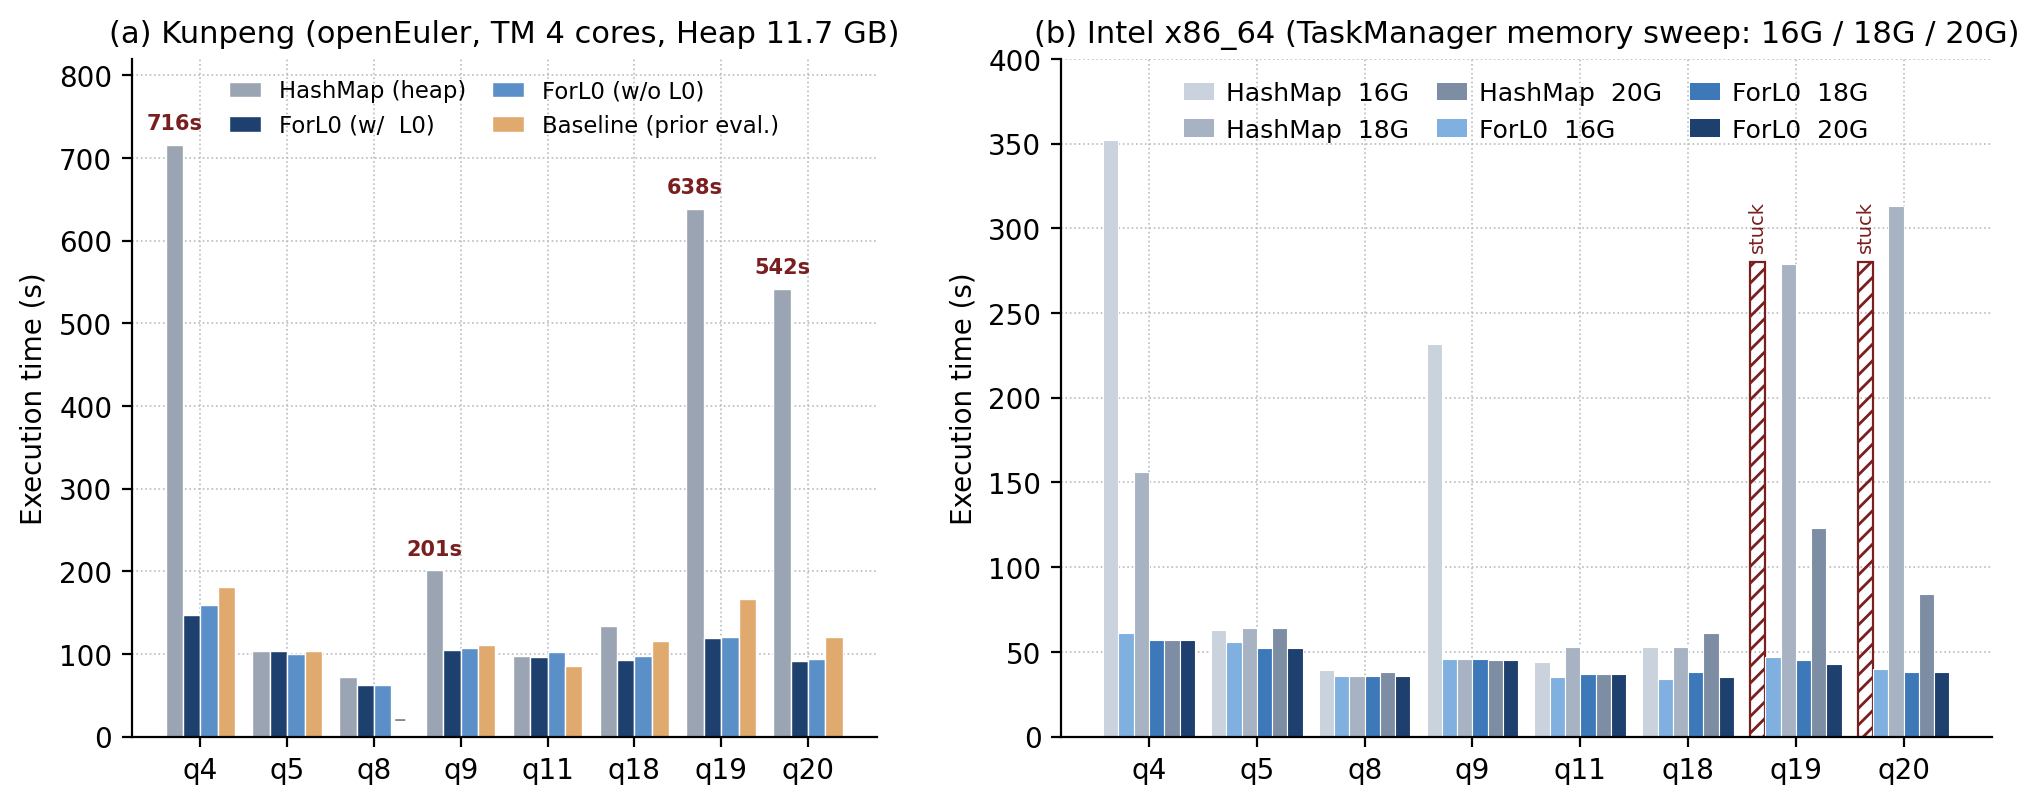
\includegraphics[width=0.98\textwidth]{nexmark_comparison.png}
  \caption{Overall performance preview based on repository results. The figure summarizes end-to-end behavior across representative NexMark queries on Kunpeng and Intel platforms, showing where \briskstate avoids the large slowdowns and stuck configurations observed with the heap baseline.}
  \Description{A two-panel bar chart comparing execution times for several NexMark queries across heap-based and \briskstate configurations on Kunpeng and Intel platforms.}
  \label{fig:preview}
\end{figure*}

Figure~\ref{fig:preview} anchors the paper with an end-to-end comparison. On both platforms, state-intensive NexMark queries show large execution-time gaps once the heap backend encounters GC pressure or memory-sensitive configurations, and the same traces can be replayed to analyze why particular queries stall or recover under a different backend.

\briskstate also remains faster at operator level. Across the 13 retained Intel \texttt{flink-state-benchmark} operations, the largest gains appear on list iteration (+132\%), map insertion (+110\%), map lookup (+91\%), value insertion (+87\%), and map removal (+74\%). Together with Figure~\ref{fig:preview}, these results connect a cheaper state path with faster full queries.

The workflow is organized in four stages:
\begin{enumerate}
  \item select a workload and switch between heap-based and cache-aware backends;
  \item observe time-series changes in throughput, tail latency, and checkpoint cost;
  \item inspect which key-groups and namespaces become hot and how occupancy evolves;
  \item replay a previously collected run to compare different execution traces.
\end{enumerate}

The workflow focuses on the causal path from data layout to locality, runtime symptoms, and externally visible metrics.

\begin{figure*}[t]
  \centering
  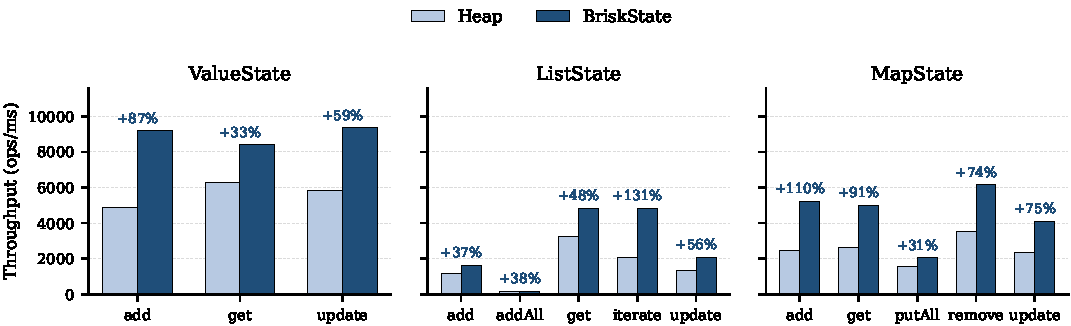
\includegraphics[width=0.9\textwidth]{flink_state_benchmark_intel.pdf}
  \caption{Operator-level Intel \texttt{flink-state-benchmark} results. \briskstate outperforms the heap backend across retained ValueState, ListState, and MapState operations.}
  \Description{A three-panel grouped bar chart showing Intel microbenchmark throughput for ValueState, ListState, and MapState operations, with \briskstate above the heap baseline and speedup labels for each operation.}
  \label{fig:microbench}
\end{figure*}

\subsection{Implementation}
The interface layer is designed to expose backend behavior without becoming a measurement artifact itself. Metrics are sampled at coarse intervals from the benchmark harness and Flink runtime, while the state view focuses on summaries such as namespace occupancy, key-group heat, and checkpoint-phase transitions.

The backend implementation also exposes details that matter for interpretation. Within each sub-table, control metadata and payload arrays are organized to support compact probing and linear snapshot traversal, and the implementation includes specialized primitive-key paths that avoid boxing for common integer and long keys. Checkpointing follows Flink's synchronous/asynchronous split: the synchronous phase captures table views using copy-on-write snapshot markers, while the asynchronous phase serializes those captured views in batches. This separation explains why checkpoint-related slowdowns sometimes appear as brief first-write penalties after a snapshot and sometimes as longer serialization tails, even when the user workload itself is unchanged.

\begin{table}[t]
  \caption{Main UI panels and the telemetry each panel explains.}
  \label{tab:panels}
  \small
  \begin{tabular}{p{0.2\columnwidth}p{0.26\columnwidth}p{0.41\columnwidth}}
    \toprule
    Panel & Data source & Purpose \\
    \midrule
    Control view & Job launcher + saved traces & How to switch workload, backend, and execution mode without leaving the same interface. \\
    Timeline & Flink runtime and checkpoint events & When throughput drops align with latency spikes or checkpoint phases instead of operator logic. \\
    State inspector & Demo collector summaries & Which key-groups and namespaces are hot, sparse, or imbalanced during the run. \\
    Comparison cards & Benchmark result summaries & Which backend is faster or more stable for the chosen scenario and why the difference is visible. \\
    \bottomrule
  \end{tabular}
\end{table}

The workflow supports both live execution and trace replay. Long-running queries and hardware-counter collection can be sensitive to machine load and deployment conditions, so the same interface can switch from streaming telemetry to recorded traces gathered from prior runs. This preserves comparability across runs while keeping the observed metrics and structural summaries in the same format.

\briskstate supports both systems analysis and operational diagnosis. It exposes state-layout design, memory locality, and execution stability at a systems level, while also making it easier to distinguish operator logic, checkpoint cadence, backend choice, and state-structure imbalance in state-intensive Flink jobs.

\section{Demonstration Scenario}
The workflow begins with a side-by-side comparison mode. One workload is executed with two different backends, and the synchronized dashboard reports throughput, latency percentiles, checkpoint cadence, and backend-specific counters. This mode establishes that backend choice changes not only final job time but also runtime stability and responsiveness.

The second stage exposes state layout directly. The interface renders a hierarchical view from operator to key-group to namespace, then overlays heat and occupancy information to show where accesses concentrate. This view shows how a smaller and more stable working set appears when namespaces are separated into compact sub-tables, and how that change affects the shape of the time-series plots.

\begin{table}[t]
  \caption{Scenarios covered in the demonstration.}
  \label{tab:scenarios}
  \small
  \begin{tabular}{p{0.18\columnwidth}p{0.23\columnwidth}p{0.46\columnwidth}}
    \toprule
    Scenario & Workload & Focus \\
    \midrule
    Pure state stress & WordCount-style updates & Observe how backend choice changes update stability, throughput, and checkpoint cadence when the state path dominates execution. \\
    Window-heavy streaming & NexMark queries & Compare how latency spikes, hot namespaces, and run-to-run variability evolve under realistic stateful pipelines. \\
    Mixed state kernels & Existing benchset jobs & Inspect interactions among ValueState, MapState, and routing structure in more application-like operators. \\
    \bottomrule
  \end{tabular}
\end{table}

\begin{figure}[t]
  \centering
  \resizebox{\columnwidth}{!}{%
  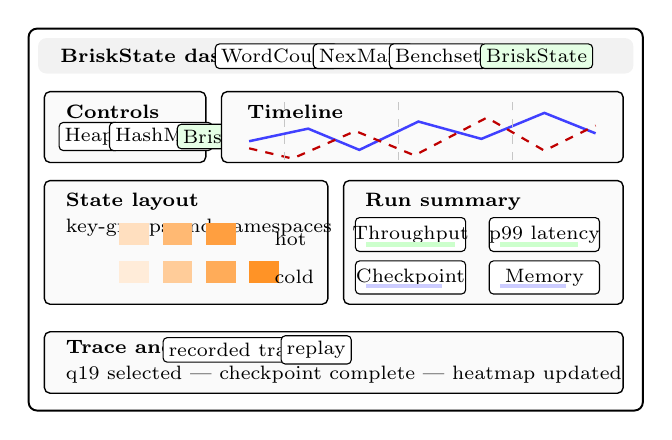
\begin{tikzpicture}[
      font=\scriptsize,
      panel/.style={draw, rounded corners=2pt, line width=0.5pt, fill=gray!4},
      title/.style={font=\scriptsize\bfseries},
      chip/.style={draw, rounded corners=1.5pt, line width=0.4pt, fill=white, inner sep=2pt},
      card/.style={draw, rounded corners=1.5pt, line width=0.4pt, fill=white}
    ]
    \draw[rounded corners=3pt, line width=0.7pt] (0,0) rectangle (7.8,4.85);
    \fill[gray!10, rounded corners=3pt] (0.12,4.28) rectangle (7.68,4.73);
    \node[anchor=west, title] at (0.28,4.5) {\briskstate dashboard};
    \node[chip] at (3.15,4.5) {WordCount};
    \node[chip] at (4.25,4.5) {NexMark};
    \node[chip] at (5.2,4.5) {Benchset};
    \node[chip, fill=green!10] at (6.45,4.5) {\briskstate};

    \draw[panel] (0.2,3.15) rectangle (2.25,4.05);
    \node[anchor=west, title] at (0.35,3.8) {Controls};
    \node[chip, anchor=west] at (0.38,3.48) {Heap};
    \node[chip, anchor=west] at (1.02,3.48) {HashMap};
    \node[chip, anchor=west, fill=green!10] at (1.88,3.48) {\briskstate};

    \draw[panel] (2.45,3.15) rectangle (7.55,4.05);
    \node[anchor=west, title] at (2.65,3.8) {Timeline};
    \draw[blue!75, line width=0.9pt] (2.8,3.42) -- (3.55,3.58) -- (4.2,3.31) -- (4.95,3.67) -- (5.75,3.45) -- (6.55,3.78) -- (7.2,3.52);
    \draw[red!75!black, dashed, line width=0.8pt] (2.8,3.33) -- (3.35,3.2) -- (4.15,3.55) -- (4.9,3.24) -- (5.82,3.72) -- (6.55,3.3) -- (7.2,3.62);
    \foreach \x in {3.25,4.7,6.15} {\draw[gray!45, dashed] (\x,3.18) -- (\x,4.0);}

    \draw[panel] (0.2,1.35) rectangle (3.8,2.92);
    \node[anchor=west, title] at (0.35,2.65) {State layout};
    \node[anchor=west] at (0.35,2.32) {key-groups and namespaces};
    \foreach \x/\y/\c in {1.15/2.1/orange!25,1.7/2.1/orange!55,2.25/2.1/orange!75,1.15/1.62/orange!15,1.7/1.62/orange!40,2.25/1.62/orange!65,2.8/1.62/orange!85} {
      \fill[\c] (\x,\y) rectangle +(0.38,0.28);
    }
    \node[anchor=west] at (3.0,2.18) {hot};
    \node[anchor=west] at (3.0,1.7) {cold};

    \draw[panel] (4.0,1.35) rectangle (7.55,2.92);
    \node[anchor=west, title] at (4.15,2.65) {Run summary};
    \draw[card] (4.15,2.02) rectangle (5.55,2.45);
    \draw[card] (5.85,2.02) rectangle (7.25,2.45);
    \draw[card] (4.15,1.48) rectangle (5.55,1.9);
    \draw[card] (5.85,1.48) rectangle (7.25,1.9);
    \node at (4.85,2.23) {Throughput};
    \node at (6.55,2.23) {p99 latency};
    \node at (4.85,1.69) {Checkpoint};
    \node at (6.55,1.69) {Memory};
    \fill[green!20] (4.28,2.08) rectangle (5.42,2.14);
    \fill[green!20] (5.98,2.08) rectangle (6.98,2.14);
    \fill[blue!20] (4.28,1.55) rectangle (5.25,1.61);
    \fill[blue!20] (5.98,1.55) rectangle (6.82,1.61);

    \draw[panel] (0.2,0.22) rectangle (7.55,1.0);
    \node[anchor=west, title] at (0.35,0.78) {Trace and replay};
    \node[chip, anchor=west] at (1.7,0.77) {recorded trace};
    \node[chip, anchor=west] at (3.2,0.77) {replay};
    \node[anchor=west] at (0.35,0.45) {q19 selected | checkpoint complete | heatmap updated};
  \end{tikzpicture}%
  }
  \caption{Interface sketch used in the paper. The layout combines workload selection, timeline comparison, state-layout inspection, run summaries, and trace replay in a single dashboard.}
  \Description{A compact dashboard schematic with a header, control chips, a timeline panel, a state-layout heatmap, four run-summary cards, and a bottom trace-and-replay strip.}
  \label{fig:ui}
\end{figure}

Figure~\ref{fig:ui} shows the interface layout. The control panel starts or replays workloads, while the timeline aligns throughput, latency, and checkpoint events. A state inspector highlights key-group and namespace occupancy, and comparison cards summarize the current run pair. The same layout also supports recorded traces collected from prior runs, so live and replayed executions remain directly comparable.

\section{Discussion and Conclusion}
State backends are central to modern stream processing, but they remain difficult to reason about because their most important properties are physical rather than logical. \briskstate combines backend structure, access locality, and runtime symptoms in a form that makes these designs easier to evaluate and reproduce. This combination of a systems prototype and a compact observation layer complements static plots by exposing parallel and memory-system behavior directly.

This paper presents \briskstate together with a lightweight observation layer. By combining the delivered native state backend, existing benchmark artifacts, workload control, synchronized metrics, and trace replay, \briskstate makes backend behavior directly observable. The result is a compact demonstration of how state layout affects stream-processing performance, stability, and debuggability.

\balance
\bibliographystyle{ACM-Reference-Format}
\bibliography{forl0-demo}

\end{document}